\begin{frame}{Введение}
    \begin{itemize}
        \item В современных компьютерных играх для реалистичной графики используют высокодетализированные модели объектов
        \item Отрисовывать все детали всех объектов на экране очень долго
        \item Классическое решение --- монолитная детализация, Level of Detail (LOD, лод)
        \item Лоды создаются вручную, это дорого
        \item Лоды сложно применять на больших объектах (зданиях, скалах)
    \end{itemize}
    \begin{center}
        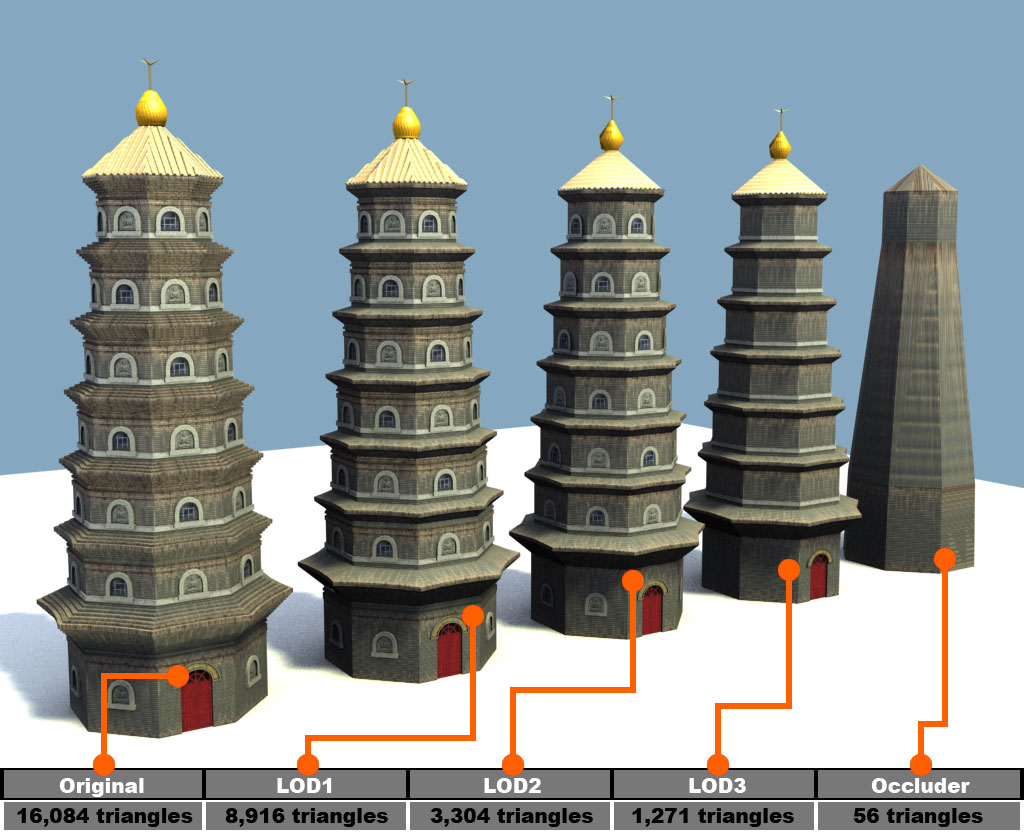
\includegraphics[height=.4\textheight]{pics/lod.jpg}
    \end{center}
\end{frame}

\begin{frame}{Альтернативы лодам}
    \begin{itemize}
        \item Geometry Clipmaps\footnote{GPU Gems 2, глава 2} --- только для ландшафта
        \item Sparse Voxel Octrees\footnote{\url{https://research.nvidia.com/sites/default/files/pubs/2010-02_Efficient-Sparse-Voxel/laine2010tr1_paper.pdf}} --- неточен, требует много памяти
        \item Nanite от Epic Games --- лучшее известное решение:
        \begin{itemize}
            \item Не нужна ручная обработка
            \item Хорошо работает на больших объектах
            \item Максимальная детализация, на которую хватает разрешения экрана
        \end{itemize}
    \end{itemize}
\end{frame}

\begin{frame}{Другие исследования}
    \begin{itemize}
        \item За 4 года никакая другая крупная компания не внедрила подобную Nanite технологию в свой движок
        \item Основные источники информации об ограничениях Nanite --- неструктурированный обмен опытом разработчиков\footnote{\url{https://www.reddit.com/r/unrealengine/comments/1697qdt/in_ue_53_what_actually_cant_be_nanite/}} \footnote{\url{https://www.reddit.com/r/unrealengine/comments/s2snhw/is_the_technology_behind_nanite_patented/}}
        \item Этого недостаточно, чтобы понять, почему технологию не реализовали в других движках
    \end{itemize}
\end{frame}

\begin{frame}{Цели и задачи}
    \textbf{Цель работы:}
    определить ограничения технологии процедурного кластерного видозависимого лоддирования и технические проблемы, которые необходимо решать при реализации

    \bigskip

    \textbf{Задачи:}
    \begin{itemize}
        \item Изучить механизм работы Nanite
        \item Реализовать упрощённую систему процедурного кластерного видозависимого изменения детализации
        \item Определить проблемы, возникающие при реализации
        \item Определить принципиальные ограничения технологии
        \item Сравнить с монолитной детализацией
    \end{itemize}
\end{frame}
